\chapter{Конструкторский раздел}
В этом разделе будет рассмотрена аппроксимация трёхмерных объектов, описаны трёхмерные преобразования,
приведены схемы разрабатываемых алгоритмов, описаны входные данные. 

\section{Аппроксимация трёхмерных объектов}
Так как пользователь может в любой момент изменить параметры объекта, то нужно предусмотреть, чтобы аппроксимация происходила автоматически.
Для цилиндра и конуса нужно выполнить следующие действия:
\begin{enumerate}
	\item Выбрать требуемое количество разбиений N для тела вращения.
	\item Подсчитать из этого угол поворота радиуса вектора для расчёта количества требуемых треугольников.
	\item Вычислить координаты следующей вершины на окружности по формуле 2.1:
	\begin{equation}
	\begin{aligned}
		& X = X_0 * Rcos(\alpha * i) \\ 
		& Y = Y_0  \\ 
		& Z = Z_0 * Rsin(\alpha * i)
	\end{aligned}
	\end{equation}
	\item Итоговая аппроксимация зависит от конкретного тела вращения. 
	Для конуса: полученные точки соединяются с вершиной. 
	Для цилиндра: из полученных точек получается прямоугольник.
\end{enumerate}

Алгоритм аппроксимации сферы сложнее. 
В программе будет генерироваться икосфера – это многогранная сфера, состоящая из треугольников \cite{ico}. 
Её преимущества в том, что она изотропна – то есть свойства тела по всем направлениям меняться не будут.
Кроме того, распределение треугольников будет равномерней, чем в других вариантах разбиения, что не будет приводить к странностям у полюсов сферы.
Поэтому алгоритм будет такой:
\begin{enumerate}
	\item На основе информации о сфере построить правильный икосаэдр, который состоит из 20 граней и 30 рёбер.
	\item Итеративно каждый треугольник икосаэдра делить на четыре одинаковых треугольника. 
	Координаты средней точки треугольника корректируются так, чтобы она лежала на сфере. 
	Процесс повторять до тех пор, пока не будет достигнута требуемая величина аппроксимации.
\end{enumerate}

На рисунке 2.1 представлен процесс итеративного приближения икосаэдра к сфере:
\FloatBarrier
\begin{figure}[h]
	\begin{center}
		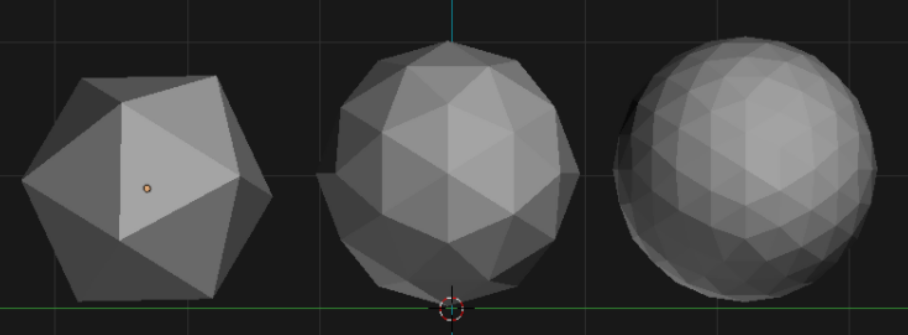
\includegraphics[width=\linewidth]{inc/ico.png}
	\end{center}
	\caption{Процесс итеративного приближения икосаэдра к сфере}
\end{figure}
\FloatBarrier

Для того, чтобы икосаэдр был сгенерирован правильно, нужно, чтобы средняя точка треугольника вычислялась с коррекцией. 
Пусть координаты средней точки треугольника – $(X_0, Y_0, Z_0)$, тогда коррекция будет выполняться по формуле 2.2:
	\begin{equation}
\begin{aligned}
& L = \sqrt{X_0^2 + Y_0^2 + Z_0^2} \\
& X_1 = \frac{X_0}{L} \\ 
& Y_1 = \frac{Y_0}{L} \\ 
& Z_1 = \frac{Z_0}{L}
\end{aligned}
\end{equation}

\section{Описание трёхмерных преобразований}

\subsection{Способ хранения декартовых координат}
Для хранения координат точек будет использоваться вектор-столбец, состоящий из четырёх координат: $ x $, $y $, $z$, $w$, причём $w$ по умолчанию равна 1. 
Это сделано для того, чтобы было удобно умножать вектор на матрицы трансформации, которые обладают размерностью 4x4.

\subsection{Преобразование трёхмерных координат в двухмерное пространство экрана}
Экран обладает только двумя координатами, поэтому нужно выбрать способ, каким образом трёхмерные объекты переносить на двухмерное пространство экрана. 
Каждый пиксель обладает определённым цветом, и за счёт этого нужно решить проблему передачи объёмности и реалистичности изображения.
Алгоритм приведения координат к нужному виду следующий:
\begin{enumerate}
	\item Перевести объект из собственного пространства в мировое.
	\item Перевести объект из мирового пространства в пространство камеры.
	\item Найти все проекции точек из пространства камеры в видимые точки, где координаты точек $ x $, $ y $ , $ z$ находятся в диапазоне [$-w$, $w$], а $w$ находится в диапазоне [0, 1].
	\item Масштабировать все точки, полученные в п.3, на картинку необходимого разрешения.
\end{enumerate}

Чтобы выполнить все преобразования, нужно использовать матрицы преобразований. 
Сначала вычисляются все необходимые матрицы, затем они перемножаются в нужном порядке. 
Исходные координаты умножаются на получившийся результат, в результате чего координаты приводятся к нужной системе.

\subsection{Преобразования трёхмерной сцены в пространство камеры}
Чтобы привести трёхмерную сцену к пространству камеру, нужно умножить каждую вершину всех полигональных моделей на матрицу камеры. 
Сама же камера задаётся аргументами: положение камеры в мировом пространстве, вектор наблюдения взгляда, направление верха камеры.
Пусть:
$\alpha$ – координаты точки в пространстве, на которую смотрит камера, 
$\beta$ – вектор, который указывает, куда смотрит верх камеры,
$\psi$– ортогональный вектор к векторам направления взгляда и вектору направления.

Тогда матрица будет выглядеть так:
\begin{equation*}
A = \left(
\begin{array}{cccc}
\alpha_x & \beta_x & \psi_x & 0\\
\alpha_y & \beta_y & \psi_y & 0 \\
\alpha_z & \beta_z & \psi_z & 0 \\
-(P*\alpha) & -(P*\beta) &-(P*\psi) & 1
\end{array}
\right)
\end{equation*}

\subsection{Матрица перспективной проекции}
После перехода в пространство камеры нужно умножить каждую вершину всех полигональных моделей на матрицу проекции. 
Эта матрица преображает заданный диапазон усечённой пирамиды в пространство отсечение, и изменяет w-компоненту так, что чем дальше от наблюдателя находится вершина, тем больше возрастает $ w $. 
После преобразования координат в пространство отсечения, координаты x и y попадают в промежуток [$-w$, $w$], а вершина $z$ – [-0, $w$]. 
Всё, что находится вне диапазона, отсекается.

Пусть AR – отношение ширины изображения к его высоте, $\alpha$ – угол обзора камеры, $Z_n$ – координата $z$ ближайшей к камере плоскости отсечения пирамиды видимости, 
$ Z_f $ – координата $z$ дальней от камеры плоскости отсечения пирамиды видимости. 
Тогда матрица перспективной проекции принимает вид:
\begin{equation*}
A = \left(
\begin{array}{cccc}
\frac{cot(\frac{\alpha}{2})}{AR} & 0 & 0 & 0\\
0 & cot(\frac{\alpha}{2}) & 0 & 0 \\
0 & 0 & \frac{Z_f \times Z_n}{Z_f - Z_n} & 1 \\
0) & 0 & \frac{Z_f}{Z_f - Z_n} & 0
\end{array}
\right)
\end{equation*}
Следующий этап – спроецировать все координаты на одну плоскость, разделив всё на координату $z$. После умножения вектора координат на матрицу перспективной проекции, реальная координата $z$ заносится в w-компоненту, так что вместо деления на $z$ делят на $w$.

\subsection{Преобразования трёхмерной сцены в пространство области изображения}
Чтобы преобразовать спроецированные координаты в координаты области изображения, нужно умножить вектор координат на матрицу. Пусть W – ширина изображения, H – высота изображения, hW – половина ширины изображения, hH – половина высоты изображения, тогда матрица преобразования сцены в пространство изображения принимает вид:

\begin{equation*}
A = \left(
\begin{array}{cccc}
hW & 0 & 0 & hW\\
0 & hH & 0 & hH \\
0 & 0 & 1 & 0 \\
0 & 0 & 0 & 1
\end{array}
\right)
\end{equation*}

\section{Алгоритм Z-буфера}
Алгоритм Z-буфера используется в первом режиме работы программы, в котором пользователь производит работу с объектами.
Совместно с алгоритмом Z-буфера применяется для закраски метод Гуро, а в качестве модели освещения используется
модель Ламберта.

На рисунке 2.2 изображена схема алгоритма Z-буфера с применением метода Гуро для закраски:
\FloatBarrier
\begin{figure}[h]
	\begin{center}
		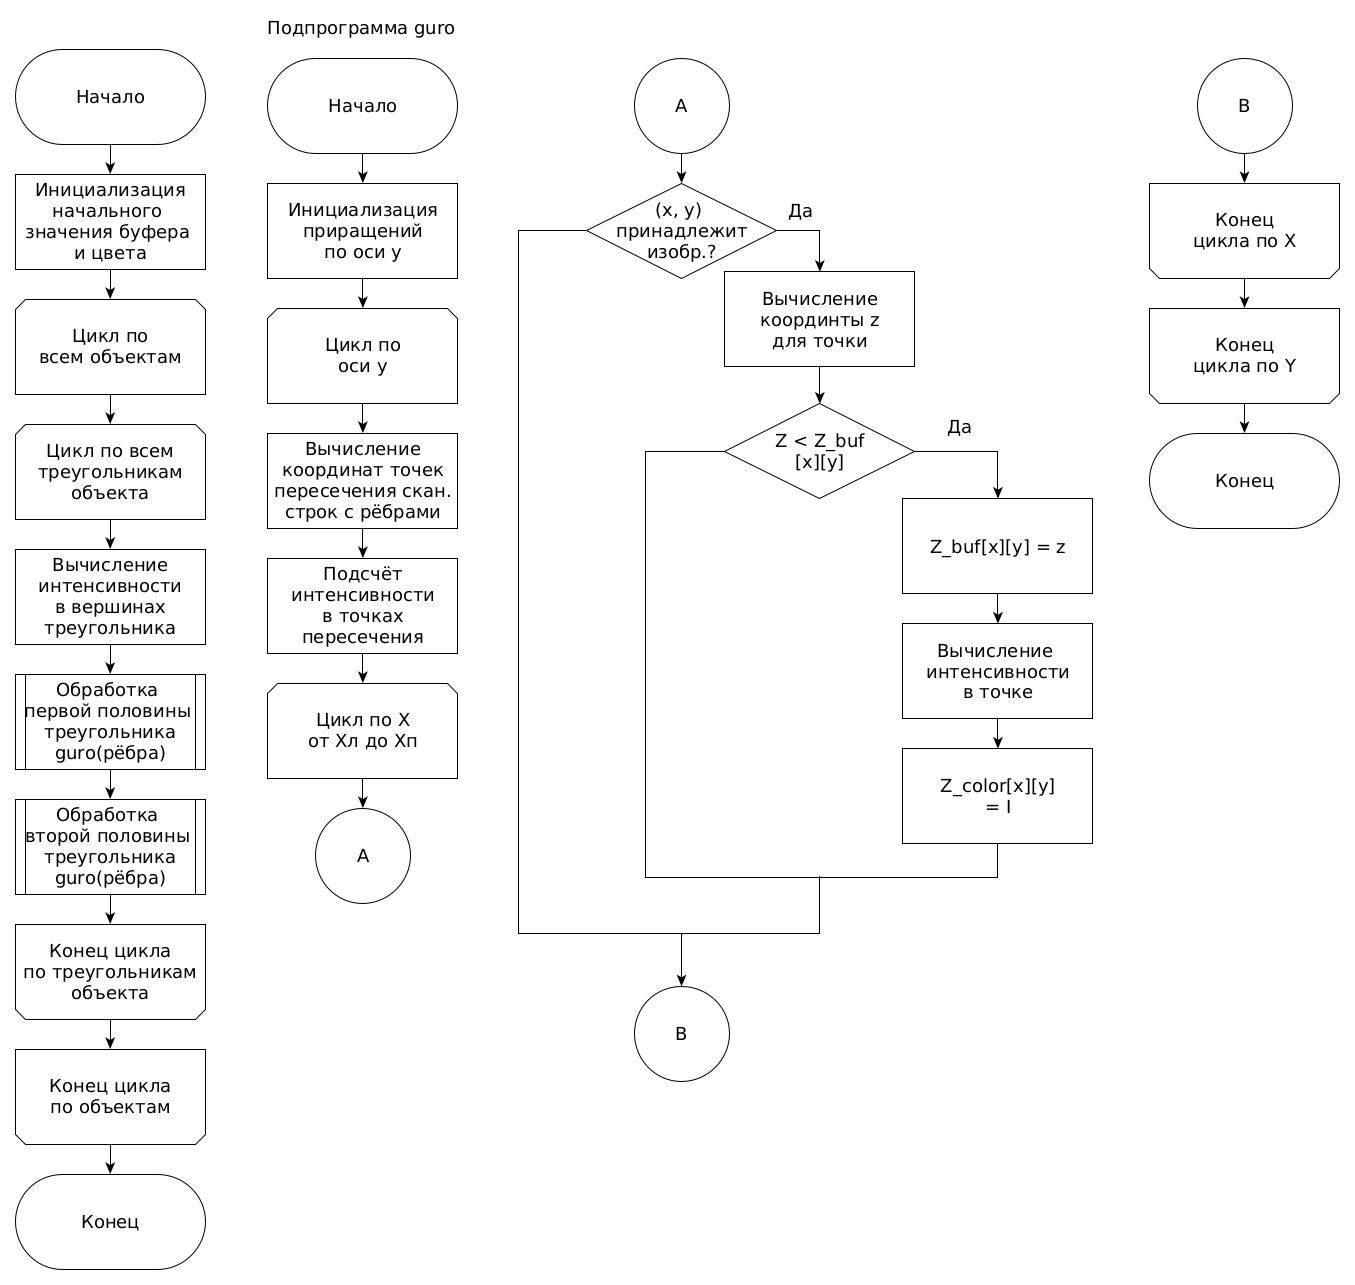
\includegraphics[width=\linewidth]{graph/zbuf.jpg}
	\end{center}
	\caption{Схема реализации алгоритма Z-буфера совместно с методом Гуро}
\end{figure}
\FloatBarrier

\section{Алгоритм обратной трассировки лучей}
Алгоритм обратной трассировки лучей используется во втором режиме работы программы для построения реалистического изображения.
Совместно с ним используется модель освещения Уиттеда.

На рисунке 2.3 приведена схема алгоритма обратной трассировки лучей.

\FloatBarrier
\begin{figure}[h]
	\begin{center}
		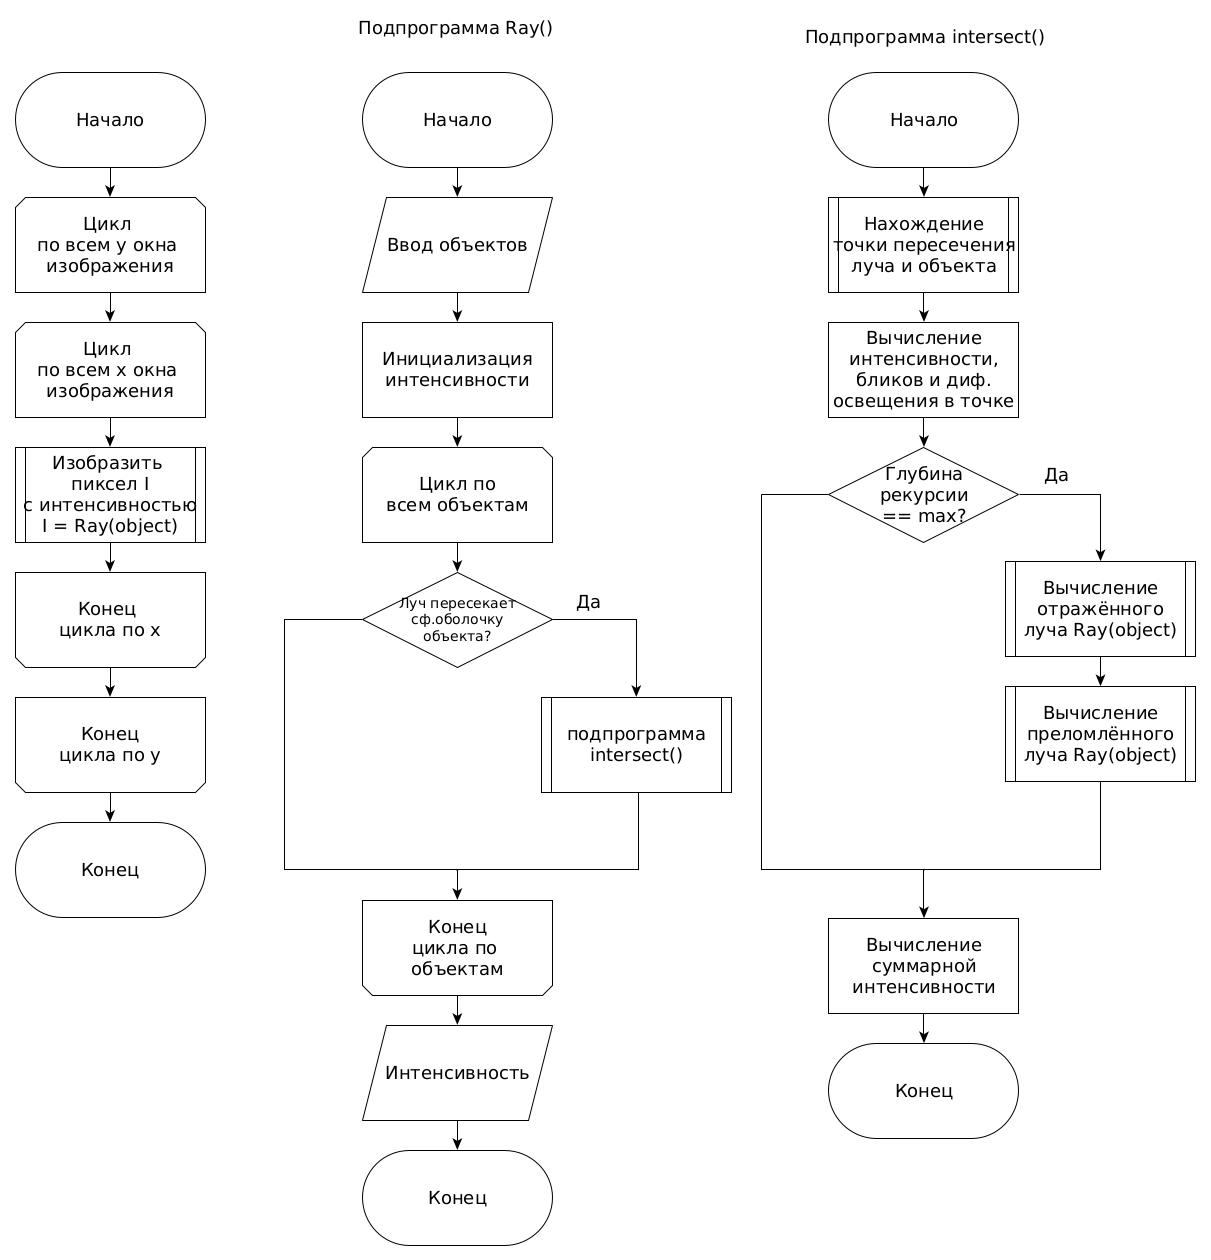
\includegraphics[width=\linewidth]{graph/tras.jpg}
	\end{center}
	\caption{Схема реализации алгоритма обратной трассировки лучей}
\end{figure}
\FloatBarrier

Для алгоритма обратной трассировки лучей нужно уметь находить отражённый и преломлённый лучи, при этом учитывая модель освещения Уиттеда.
Отражённый луч можно найти, зная направление падающего луча и нормаль к поверхности. 

Пусть $ \overline{L} $ -- направление луча, а $ \overline{n} $ – нормаль к поверхности. 
Луч можно разбить на две части: , $ \overline{L_p} $ которая перпендикулярна нормали, и  $ \overline{L_n} $ – параллельна нормали.

Представленная ситуация изображена на рисунке 2.4:
\FloatBarrier
\begin{figure}[h]
	\begin{center}
		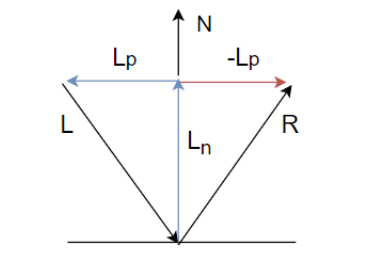
\includegraphics[]{inc/vecs.png}
	\end{center}
	\caption{Рассматриваемые векторы для расчёта отражённого луча.}
\end{figure}
\FloatBarrier

Учитывая свойства скалярного произведения $ \overline{L_n} = \overline{n} * (\overline{n}, \overline{L}) $ и  $ \overline{L_p} = \overline{L} - \overline{n} * (\overline{n}, \overline{L}) $
Так как отражённый луч выражается через разность этих векторов, то отражённый луч выражается по формуле 2.3:
\begin{equation}
R = 2*\overline{n}*(\overline{n}, \overline{L}) - \overline{L}
\end{equation}

По закону преломления падающий, преломлённый луч и нормаль к поверхности лежат в одной плоскости. 
Пусть $ \mu_i$ -- показатели преломления сред, а $\eta_i$ – углы падения и отражения света соответственно. 
Применяя закон Снеллиуса, параметры преломлённого луча можно вычислить по формуле 2.4:
\begin{equation}
\begin{aligned}
& R = \frac{\mu_1}{\mu_2} \overline{L} + ( \frac{\mu_1}{\mu_2} cos(\eta_1) - cos(\eta_2))\overline{n} \\ 
& cos(\eta_2) = \sqrt{1 - (\frac{\mu_1}{\mu_2})^2 * (1 - cos(\eta_1))^2}
\end{aligned}
\end{equation} 

\section{Алгоритм пересечения луча с параллелепипедом}
При работе алгоритма обратной трассировки лучей крайне неэффективно при каждой трассировке луча искать пересечения со всеми полигонами каждого объекта в сцене, поэтому имеет смысл заключить объект в параллелепипед, который бы полностью его включал.

Данный параллелепипед задаётся координатами двух вершин: с минимальными и максимальными значениями координат $ x $, $ y $, $ z $. Таким образом это позволяет задать шесть плоскостей, ограничивающих параллелепипед, и при этом все они будут параллельны координатным плоскостям.

Рассмотрим пару плоскостей, параллельных плоскости yz: X = x1 и X = x2. Пусть $ \overline{D} $ -- вектор направления луча. Если координата $ x $ вектора $ D $ равна 0, то заданный луч параллелен этим плоскостям, и, если $ x_0 < x_1 $ или $ x_0 > x_1 $, то он не пересекает рассматриваемый прямоугольный параллелепипед. Если же Dx не равно 0, то вычисляются отношения 2.5: 

\begin{equation}
\begin{aligned}
& t_{1x} = \frac{x_1 - x_0}{D_x} \\ 
& t_{2x} = \frac{x_2 - x_0}{D_x} \\
\end{aligned}
\end{equation} 

Можно считать, что найденные величины связаны неравенством $ t_{1x} < t_{2x} $.
Пусть $t_n = t_{1x}$, $t_f = t_{2x}$. Считая, что $D_y$ не равно нулю, и рассматривая вторую пару плоскостей, несущих грани заданного параллелепипеда, $Y = y_1$, $Y = y_2$, вычисляются величины:

\begin{equation}
\begin{aligned}
& t_{1y} = \frac{y_1 - y_0}{D_y} \\ 
& t_{2y} = \frac{y_2 - y_0}{D_y} \\
\end{aligned}
\end{equation} 

Если $t_{1y} > t_n$, то тогда $t_n = t_{1y}$.
Если $t_{2y} < t_f$, то тогда $t_f = t_{2y}$.
При $t_n > t_f$ или при $t_f < 0$ заданный луч проходит мимо прямоугольного параллелепипеда.

Считая, что $D_z$ не равно нулю, и рассматривая вторую пару плоскостей, несущих грани заданного параллелепипеда, $Z = z_1$, $Z = z_2$, вычисляются величины:

\begin{equation}
\begin{aligned}
& t_{1z} = \frac{z_1 - z_0}{D_z} \\ 
& t_{2z} = \frac{z_2 - z_0}{D_z} \\
\end{aligned}
\end{equation} 
и повторяются сравнения, приведённые для формулы 2.6.

Если в итоге всех проведённых операций получается, что $0 < t_n < t_f$ или $ 0 < t_f$, то заданный луч пересечёт исходный параллелепипед со сторонами, параллельными координатным осям.

Следует отметить, что при пересечении лучом параллелепипеда извне знаки $t_n$ и  $t_f$ должны быть равны, в противном случае можно сделать вывод, что луч пересекает параллелепипед изнутри.

\section{Описание входных данных}
В разработанной программе входные данные подаются в виде файла с расширением .obj. В этом формате помимо координат вершин можно передавать информацию о текстурах и нормалях.

Формат файла:
\begin{enumerate}
	\item Список вершин с координатами $(x, y, z)$:
		
		v 0.56 0.19 -1.32
	\item Текстурные координаты $(u, v)$:
		
		vt 0.430 0.2
	\item Координаты нормалей $(x, y, z)$:
		
		vn 0.5 -1 -0.2
	\item Определение поверхности задаётся в формате i1/i2/i3, где i1 -- индекс координаты вершины, i2 -- индекс координаты текстуры, i3 -- индекс координаты нормали:
		
		f 1/3/5 2/4/6 3/9/7
\end{enumerate}

\section{Вывод}
В этом разделе была рассмотрена аппроксимация трёхмерных объектов, описаны трёхмерные преобразования,
приведены схемы разрабатываемых алгоритмов, описаны входные данные. 